\chapter{Implementing policy-agnostic programming on the client side\label{chap:solution}}
We incorporated policy-agnostic programming into Javascript by adding constructs
defined for the Jeeves language as a subsystem. We chose Narcissus~\cite{narc},
a Javascript interpreter written in Javascript, to create the proof of concept.
Narcissus was built by its developers to be able to prototype new language features
for Javascript.

\section{Implementing faceted values in Narcissus}
Integral to implementing Jeeves is the implementation of faceted values. Our implementation
of faceted values derives heavily from the work done by Austin and Flanagan~\cite{Faceted}
and is inspired from the concept presented by Kerchove et al~\cite{Modular} for
``modular instrumentation'' of interpreters. They talk about how many dynamic analysis
approaches for information flow security have prototypes that are implemented in
very specific ways making it difficult to compare and reuse. They derive some
specific criteria to follow in order to achieve ``modular instrumentation'' using
the implementation of~\cite{Faceted} as a case study. While we borrow a few ideas
from this, our implementation does not follow the criteria specified because achieving
``modular instrumentation'' would involve non-trivial changes to the Narcissus
interpreter making it out of scope of our problem. What we did achieve is untangling
of the concerns of the core interpreter for non-faceted evaluation from the concerns
of faceted evaluation. This makes it easier to relate principles of faceted evaluation
with the implemented prototype and also to extend or reuse it.

Our implementation of faceted values is independent from the core Narcissus interpreter.
This involved making the core interpreter modular to be able to modify existing
evaluation mechanisms to behave differently for faceted values. The Narcissus interpreter
has an execute function which consists a switch case control flow that is set to
perform the appropriate set of operations based on the type of node identified by
the parser. Wherever there is need for faceted behavior, instead of making the core
interpreter code handle faceted behavior, we moved the part we would need to change
into a method and later override the method to handle faceted behavior.
Figure~\ref{fig:facetif} shows how this overriding is implemented for the [F-IF-SPLIT]
evaluation rule. Here, \texttt{BaseExecContext} is an object that stores a copy of all the
methods from the core interpreter which we need to override. \texttt{ExecutionContext}
is an object from the core interpreter that keeps track of the current flow of execution.
\texttt{FacetExecContext} is the \texttt{ExecutionContext} object extended with
the \textit{pc} to help keep track of the influence of public or private facets
on the current flow of execution. In the \texttt{evalIfBlock} function, notice we
call the base \texttt{evalIfBlock} function if \texttt{cond} is not a faceted value.
Otherwise, we call the \texttt{evaluateEach} function which encapsulates all the
function application rules from Figure\ref{fig:appRules}. Similarly, we override
the rest of the functions in \texttt{BaseExecContext}.
\lstset{
  language=javascript,
  frame=single,
  breaklines=true,
  basicstyle=\footnotesize\ttfamily,
  numbers=left,
  extendedchars=true,
  tabsize=2
}
\begin{figure}
  \begin{lstlisting}
var BaseExecContext = {
  getValue: interpreter.ExecutionContext.prototype.getValue,
  putValue: interpreter.ExecutionContext.prototype.putValue,
  evalBinOp: interpreter.ExecutionContext.prototype.evalBinOp,
  evalUnaryOp: interpreter.ExecutionContext.prototype.evalUnaryOp,
  evalIfBlock: interpreter.ExecutionContext.prototype.evalIfBlock
};

FacetExecContext.prototype.evalIfBlock = function(cond,thenPart,elsePart) {
  var execContext = FacetExecContext.current;
  if (cond instanceof FacetedValue) {
    evaluateEach(cond, function(v, x) {
      if (v) {
        interpreter.execute(thenPart, x);
      } else if (elsePart) {
        interpreter.execute(elsePart, x);
      }
    }, execContext);
  } else {
    BaseExecContext.evalIfBlock.call(this,cond,thenPart,elsePart);
  }
};
  \end{lstlisting}
  \caption{Independent implementation of faceted behavior for the ``if'' control flow}
  \label{fig:facetif}
\end{figure}

\begin{figure}
  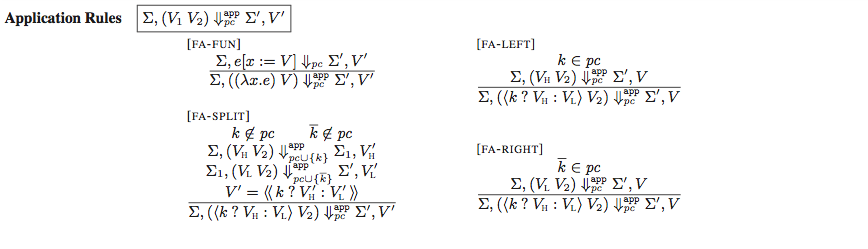
\includegraphics[scale=0.5, frame]{images/appRules}
  \caption{Function application rules~\cite{FacetedJeeves}}
  \label{fig:appRules}
\end{figure}

\section{Implementing Jeeves}
Once we had faceted values working, adding support for Jeeves constructs was pretty
straightforward. All of the Jeeves constructs are encapsulated in the prototype
of the \texttt{PolicyEnvironment} object which includes the [F-LABEL] and [F-RESTRICT]
evaluation rules as shown in Figure~\ref{fig:jeevesEval}. Every instance of the \texttt{PolicyEnvironment}
object has a \texttt{policyMap} that is used to store the `label':`policy' mapping.

\begin{figure}
  \centering
  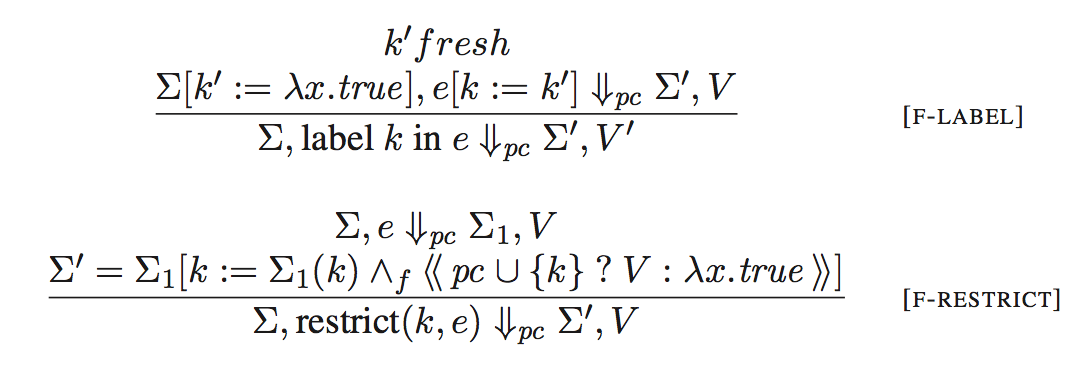
\includegraphics[scale=0.3]{images/jeevesEval}
  \caption{Evaluation semantics for Jeeves labels and policies~\cite{FacetedJeeves}}
  \label{fig:jeevesEval}
\end{figure}

The Jeeves constructs available in the \texttt{PolicyEnvironment} prototype are:
\begin{enumerate}
  \item \texttt{mkLabel:} This method is roughly based on the [F-LABEL] rule. It
    creates a label and associates a default true policy to it.
  \item \texttt{restrict:} This method associates the given policy function to the
  given label in the \texttt{policyMap} of the current \texttt{PolicyEnvironment}.
  \item \texttt{mkSensitive:} This method creates a faceted value. It takes the
  label, private value, and public value as input and returns a faceted value. This
  method would only return the private value or the public value in cases where
  the current program counter contains the label or reverse of the label respectively.
  \item \texttt{concretize:} This method is used when the faceted value needs to
  be viewed in an output context. It takes the context object and faceted value
  as input and resolves the policies for all labels in the program counter of
  the faceted value recursively till it reaches a raw value with no facets.
  \item \texttt{partialConcretize:} Partial concretize is similar to the concretize
  function except it only resolves the policy associated with the first label of
  a possibly complex faceted value based on the given context object.
  Figure~\ref{fig:concretize} shows what the concretize and partialConcretize
  functions look like.
\end{enumerate}

\begin{figure}
  \begin{lstlisting}
function concretize(context, val) {
  if (val instanceof FacetedValue) {
    var label = head(val);
    var policy = this.policyMap[label];
    if (policy(context)) {
      return this.concretize(context, val.high);
    } else {
      return this.concretize(context, val.low);
    }
  } else {
    return val;
  }
}
function partialConcretize(context, val) {
  if (val instanceof FacetedValue) {
    var label = head(val);
    var policy = this.policyMap[label];
    if (policy(context)) {
      val = val.high;
    } else {
      val = val.low;
    }
  }
  return val;
}
  \end{lstlisting}
  \caption{Concretize and partialConcretize function definitions}
  \label{fig:concretize}
\end{figure}

\subsection{Usage of the Jeeves constructs}
Figure~\ref{fig:JeevesExamples} shows two test cases of how the Jeeves constructs
listed above would be used. Note, \texttt{policyEnv} is an instance of the
\texttt{PolicyEnvironment} prototype.

In \texttt{testPolicyComplexFacets}, we are constructing complex faceted values
with two principals/labels and have two different policies for each respectively.
The call to \texttt{concretize} at the end shows what a context object would look
like in this case. The faceted value stored in \texttt{a} in notation looks like
this: $\langle x~?~\langle y~?10~:~15 \rangle~:~0 \rangle$.

In \texttt{testPartialConcretize}, we are using \texttt{partialConcretize} with
two different context objects. This type of usage would be ideal for a client-server
interaction where you can have different context objects for the server and client-side
respectively. Note, in the example the policies associated with the two labels are
expecting different properties in the context object passed to them.

\begin{figure}
  \begin{lstlisting}
 function() testPolicyComplexFacets{
  var x = policyEnv.mkLabel("x");
  policyEnv.restrict(x, function (context) {
    return context.val1 === 22 && context.val2 === 21;
  });

  var y = policyEnv.mkLabel("y");
  policyEnv.restrict(y, function (context) {
    return context.val2 === 22;
  });
  var a = policyEnv.mkSensitive(x, policyEnv.mkSensitive(y, 10, 15), 0);
  return assertEquals(policyEnv.concretize({val1: 22, val2: 21}, a), 15);
};

function testPartialConcretize() {
  var x = policyEnv.mkLabel("x");
  policyEnv.restrict(x, function (context) {
    return context.val1 === 22 && context.val2 === 21;
  });

  var y = policyEnv.mkLabel("y");
  policyEnv.restrict(y, function (context) {
    return context.otherVal = 44;
  });
  var a = policyEnv.mkSensitive(x, policyEnv.mkSensitive(y, 10, 15), 0);

  var result1 = assertEquals(policyEnv.partialConcretize({val1: 22, val2: 21}, b).toString(), "{y?10:15}");
  var result2 = assertEquals(policyEnv.partialConcretize({val:22}, b), 0);
  return result2 && result1;
};
  \end{lstlisting}
  \caption{Example usage of Jeeves constructs}
  \label{fig:JeevesExamples}
\end{figure}

\textbf{\textit{Should i move the following sections to their own separate chapter?}}
\section{Policy agnostic programming in dom.js}
With Jeeves constructs in place, we now demonstrate how policy-agnostic programming
will help protect browser content. We do that by building policy-agnostic programming
controls into dom.js which is a Javascript DOM implementation~\cite{dom.js}. There
were a few challenges to get dom.js to work with Narcissus. The primary obstacle
was that dom.js heavily depended on prototype inheritance but Narcissus in its
original form did not support it. We added prototype inheritance support to our
version of Narcissus and got dom.js working.

\section{A data-exfiltration case study}


\textbf{\textit{This is a work in progress...}}
% Our original intention was to integrate our version of Narcissus into a web browser
% and replace the host Javascript engine.
